% !TeX program = pdflatex
% La firma de Fourier por voz: el bajo es la voz espectralmente más pura.
% Versión en español (traducción con sentido del original en inglés, per_voice_note.tex).
% Autor: Carles Marin (con Claude, Anthropic, como asistente de IA).
% Build: pdflatex per_voice_note_es.tex (dos veces, por las referencias). Figuras: figs/*.pdf

\documentclass[11pt]{article}
\usepackage[T1]{fontenc}
\usepackage[spanish,es-noindentfirst,es-noshorthands]{babel}
\usepackage{lmodern}
\usepackage{amsmath,amssymb,amsthm,booktabs,graphicx}
\usepackage[hidelinks]{hyperref}
\usepackage{xurl}
\usepackage[table]{xcolor}
\usepackage[margin=1in]{geometry}
\usepackage{microtype}
\usepackage{float}
\usepackage{placeins}
\usepackage{tikz}
\usetikzlibrary{arrows.meta,positioning,calc}
\definecolor{ctA}{HTML}{1B6F8C} % el acento "estructural / puro"
\definecolor{ctB}{HTML}{B5530F} % el acento "cromático / color"
\setlength{\emergencystretch}{2em}
% colocación de floats -- empaquetar floats en páginas de texto, minimizar huecos
\renewcommand{\topfraction}{0.92}
\renewcommand{\bottomfraction}{0.85}
\renewcommand{\textfraction}{0.08}
\renewcommand{\floatpagefraction}{0.75}
\setcounter{topnumber}{3}
\setcounter{bottomnumber}{2}
\setcounter{totalnumber}{4}
\raggedbottom % recoger el espacio sobrante al pie en vez de estirarlo en medio de la página
\newtheorem{theorem}{Teorema}
\newtheorem{proposition}{Proposición}
\newtheorem{lemma}{Lema}
\newtheorem{remark}{Observación}
\newcommand{\lean}[1]{\texttt{#1}}
\newcommand{\Ztwelve}{\mathbb{Z}_{12}}
\newcommand{\Zn}[1]{\mathbb{Z}_{#1}}
\newcommand{\Ahat}{\hat{A}}
\newcommand{\question}[1]{\smallskip\noindent\textit{#1}\smallskip}
\newcommand{\audiobase}{https://github.com/karlesmarin/music-math/raw/main/media}
\newcommand{\audio}[1]{\href{\audiobase/#1}{\textcolor{ctA}{\footnotesize\,[$\flat$\,audio]}}}

\title{\bf La firma de Fourier por voz:\\ el bajo es la voz espectralmente más pura}
\author{Carles Mar\'in Mu\~noz\thanks{Preparado con la asistencia de un sistema de IA (Claude, Anthropic).
La matemática es clásica y el hallazgo central es empírico; toda afirmación, delimitación de alcance y
limitación es responsabilidad del autor. La frontera de la contribución se enuncia con claridad en la
Sección~\ref{sec:novelty}, y es el núcleo de Lean~4 ---no el asistente--- lo que certifica la parte
formalizada (Sección~\ref{sec:checked}).}\\[3pt]
  \normalsize Investigador independiente\\
  \normalsize \texttt{karlesmarin@gmail.com}}
\date{Junio de 2026\\[3pt]\normalsize DOI: \href{https://doi.org/10.5281/zenodo.20971090}{10.5281/zenodo.20971090}
\quad\textbullet\quad \href{https://github.com/karlesmarin/music-math}{github.com/karlesmarin/music-math}}

\begin{document}
\maketitle

\begin{abstract}\noindent
Durante tres siglos la teoría musical ha sostenido que el bajo es especial ---la \emph{basse fondamentale}
de Rameau, la tradición del bajo cifrado, las funciones armónicas de Riemann: la voz más grave porta las
raíces armónicas, el fundamento. Eso siempre fue una afirmación \emph{estructural}. La transformada de
Fourier discreta de distribuciones de clases de altura (Lewin, Quinn, Amiot, Yust) convirtió las
``cualidades'' de los acordes en números ---la magnitud $|a_k|$ del $k$-ésimo coeficiente mide un carácter:
$|a_5|$ diatonicidad, $|a_1|$ cromaticidad, $|a_6|$ tonalentereza. Ese programa lee una pieza por
\emph{tiempo}; nunca ha preguntado si cada \emph{voz} porta una huella espectral distinta. Aquí lo hacemos.
Sobre $334$ corales de Bach a cuatro voces, la conjetura ingenua ---que el bajo, que camina por quintas, es
la voz más diatónica ($|a_5|$)--- es \emph{falsa} (lo es la soprano). Pero el dato muestra algo más
afilado: el \textbf{bajo es la voz espectralmente más pura}, la más baja en cromaticidad
($\alpha_1=|a_1|/|a_0|$, pareado $t=-20$) y en tonalentereza ($\alpha_6$, $t=-15$), \emph{a pesar de usar
el vocabulario de clases de altura más amplio} ---así que no es un artefacto de cardinalidad. La causa es
la \textbf{realización de raíces} actuando por dos canales: las raíces funcionales se mueven por
quintas/cuartas (intervalos impares), que equilibran el peso par/impar y llevan $\alpha_6\!\to\!0$ (el
canal de \emph{paridad}), y la amplia tesitura del bajo dispersa su peso por el círculo cromático, bajando
$\alpha_1$ (el canal de \emph{dispersión}). El efecto está \textbf{acotado por la textura}: fuerte en la
homofonía de bajo funcional (corales de Bach; Palestrina), se desvanece en texturas imitativas (madrigales
de Monteverdi) y prefuncionales (Trecento) ---de modo que la firma es un \emph{diagnóstico de la escritura
de bajo funcional}, y el límite confirma el mecanismo. El núcleo del canal de paridad ---que $a_6$ es la
imbalancia de paridad par-menos-impar--- está verificado por máquina en Lean~4 (\lean{ParityA6.lean},
sin \lean{sorry}, axiom-clean, universo par general). Todo ingrediente es clásico (el bajo funcional de
Rameau/Riemann; $a_6=$ paridad de clases, Amiot; la regla del movimiento de una sola nota, Hoffman); la
contribución es la \textbf{ley de magnitud por voz} ---un hecho medido, explicado, certificado y
honestamente acotado--- no matemática nueva.
\end{abstract}

\section{¿Es el bajo realmente el fundamento?}\label{sec:hook}

Cuando Jean-Philippe Rameau situó la \emph{basse fondamentale} en el centro de la armonía en
1722~\cite{Rameau}, precisó un viejo instinto práctico: la voz más grave no es una melodía más, sino la
portadora de las raíces de los acordes, el suelo sobre el que se sostiene la armonía. La tradición del
bajo cifrado codificó la misma prioridad, y las funciones armónicas de Hugo Riemann~\cite{Riemann} leyeron
después el movimiento tonal como una lógica de funciones enraizadas en el bajo. ``El bajo es el fundamento''
se volvió una de las afirmaciones más duraderas de la teoría musical ---y siguió siendo \emph{estructural},
cualitativa.

Ese instinto fue, durante siglo y medio, también una práctica diaria. En el \emph{basso continuo} barroco,
una sola línea de bajo ---anotada con cifras--- bastaba para que un teclista realizara toda una armonía,
derivándose las voces superiores del bajo y no al revés. La \emph{basse fondamentale} de Rameau dio a la
práctica una teoría: bajo el bajo sonante yace una línea conceptual de \emph{raíces} de acorde, y la armonía
es el movimiento de esa línea; Riemann recompuso después ese movimiento como una gramática compacta de
funciones de tónica, subdominante y dominante, de nuevo ancladas abajo. A lo largo de la práctica común,
pues, el bajo quedó señalado por triplicado ---en la interpretación, en la teoría y en la pedagogía---
como la voz que \emph{define} la armonía. La afirmación estaba en todas partes; un número para ella, en
ninguna.

Dos siglos y medio después de Rameau, David Lewin~\cite{Lewin1959} ---en una nota de dos páginas de 1959 hoy
vista como la semilla de todo el tema--- empezó a convertir la estructura interna de los acordes en
coeficientes de Fourier, idea revivida por Ian Quinn como una teoría de la ``cualidad'' de los
acordes~\cite{Quinn} y convertida en disciplina por Emmanuel Amiot~\cite{Amiot} y Jason
Yust~\cite{Yust2017,Yust2019}. Se codifica un acorde o un pasaje como
una distribución sobre las doce clases de altura $\Ztwelve$, se toma su transformada de Fourier discreta, y
las \emph{magnitudes} $|a_k|$ se leen como \textbf{caracteres} musicales: $|a_5|$ es diatonicidad, $|a_4|$
octatonicidad, $|a_6|$ tonalentereza, $|a_1|$ cromaticidad. El perfil de caracteres de una pieza puede
seguirse, graficarse, hasta dibujarse como un diagrama de sectores. Pero todo análisis en este programa
segmenta la textura por \emph{tiempo} ---ventanas deslizantes sobre la distribución de clases de altura de
toda la textura. \textbf{Ninguno ha preguntado lo ortogonal: ¿porta cada voz, por su papel registral, un
perfil de carácter de Fourier distinto?}

Esta nota sigue esa única pregunta. Nos permite poner la intuición estructural de Rameau sobre un
instrumento de medida: si el bajo es de verdad el fundamento armónico, debería dejar una \emph{huella}
espectral medible, distinta de las voces que tiene encima. La deja ---pero no la huella que uno adivinaría
primero, y solo exactamente donde la armonía es funcional.

\section{Preliminares: la DFT por voz}\label{sec:setup}

Fijada una voz $v$ en una pieza, formamos su \textbf{distribución de clases de altura ponderada por
duración} $\mu_v:\Ztwelve\to\mathbb{R}_{\ge 0}$, donde $\mu_v(x)$ es la duración sonante total que la voz
pasa en la clase de altura $x$ (octava colapsada). Su transformada de Fourier discreta es
\[
  a_k(v)\;=\;\hat\mu_v(k)\;=\;\sum_{x\in\Ztwelve}\mu_v(x)\,e^{-2\pi i\,kx/12},\qquad k=0,1,\dots,6,
\]
con $a_0=$ peso total. Comparamos voces por el \textbf{carácter normalizado}
$\alpha_k(v)=|a_k(v)|/|a_0(v)|\in[0,1]$, invariante a cuán fuerte o larga sea la voz. Los caracteres con
nombre son los estándar~\cite{Amiot,Yust2019}: $\alpha_1$ cromático, $\alpha_2$ cuartal, $\alpha_3$
aumentado, $\alpha_4$ octatónico, $\alpha_5$ diatónico, $\alpha_6$ tono-entero. Las voces se identifican por
\emph{registro} (altura media), de modo que ``bajo'' es la parte más grave y ``soprano'' la más aguda
---sin depender de nombres de partes. Toda la construcción es lineal en la descomposición en voces; la
contribución aquí es empírica, en lo que revela la medición.

\section{La primera apuesta, y la sorpresa}\label{sec:law}

\question{P\textsubscript{1}. El bajo camina por quintas y porta las raíces ---¿es entonces la voz más
generada-por-quintas, es decir, la más \emph{diatónica} ($\alpha_5$)?}

Es una apuesta natural, y es \textbf{falsa}. Sobre los $334$ corales a cuatro voces de J.S.~Bach (corpus de
\lean{music21}), la soprano es la voz más diatónica ($\alpha_5=0{,}580$ frente al $0{,}535$ del bajo,
pareado $t=-10{,}4$). El bajo no es donde la diatonicidad alcanza su máximo.

Lo que la medición \emph{sí} revela es más afilado y más robusto. El bajo es la voz \textbf{espectralmente
más pura}: la más baja en cromaticidad $\alpha_1$ y la más baja en tonalentereza $\alpha_6$, por amplio
margen (Figura~\ref{fig:camembert}; la tabla es la Figura~\ref{fig:heatmap}). Medias por voz, Bach:

\begin{center}\small
\begin{tabular}{@{}lcccccc@{}}
\toprule
\textbf{voz} & $\alpha_1$ crom & $\alpha_2$ & $\alpha_3$ & $\alpha_4$ oct & $\alpha_5$ diat & $\alpha_6$ t-ent\\
\midrule
Bajo    & \textbf{0{,}130} & 0{,}207 & 0{,}257 & 0{,}118 & 0{,}535 & \textbf{0{,}079}\\
Tenor   & 0{,}279 & 0{,}181 & 0{,}261 & 0{,}186 & 0{,}525 & 0{,}190\\
Alto    & 0{,}363 & 0{,}233 & 0{,}298 & 0{,}197 & 0{,}505 & 0{,}223\\
Soprano & 0{,}297 & 0{,}170 & 0{,}233 & 0{,}183 & \textbf{0{,}580} & 0{,}216\\
\bottomrule
\end{tabular}
\end{center}

Pareado contra la soprano: $\alpha_1$ $t=-20{,}3$, $\alpha_6$ $t=-14{,}8$ ---los dos mayores efectos de la
tabla. \textbf{El bajo es la voz menos cromática y menos tono-entero; la soprano es la más diatónica; las
voces internas son las más cromáticas.} Puede oírse el contraste: el bajo de un coral solo
\audio{bwv66_6_bass.wav} frente a su alto \audio{bwv66_6_alto.wav}.

\begin{figure}[H]\centering
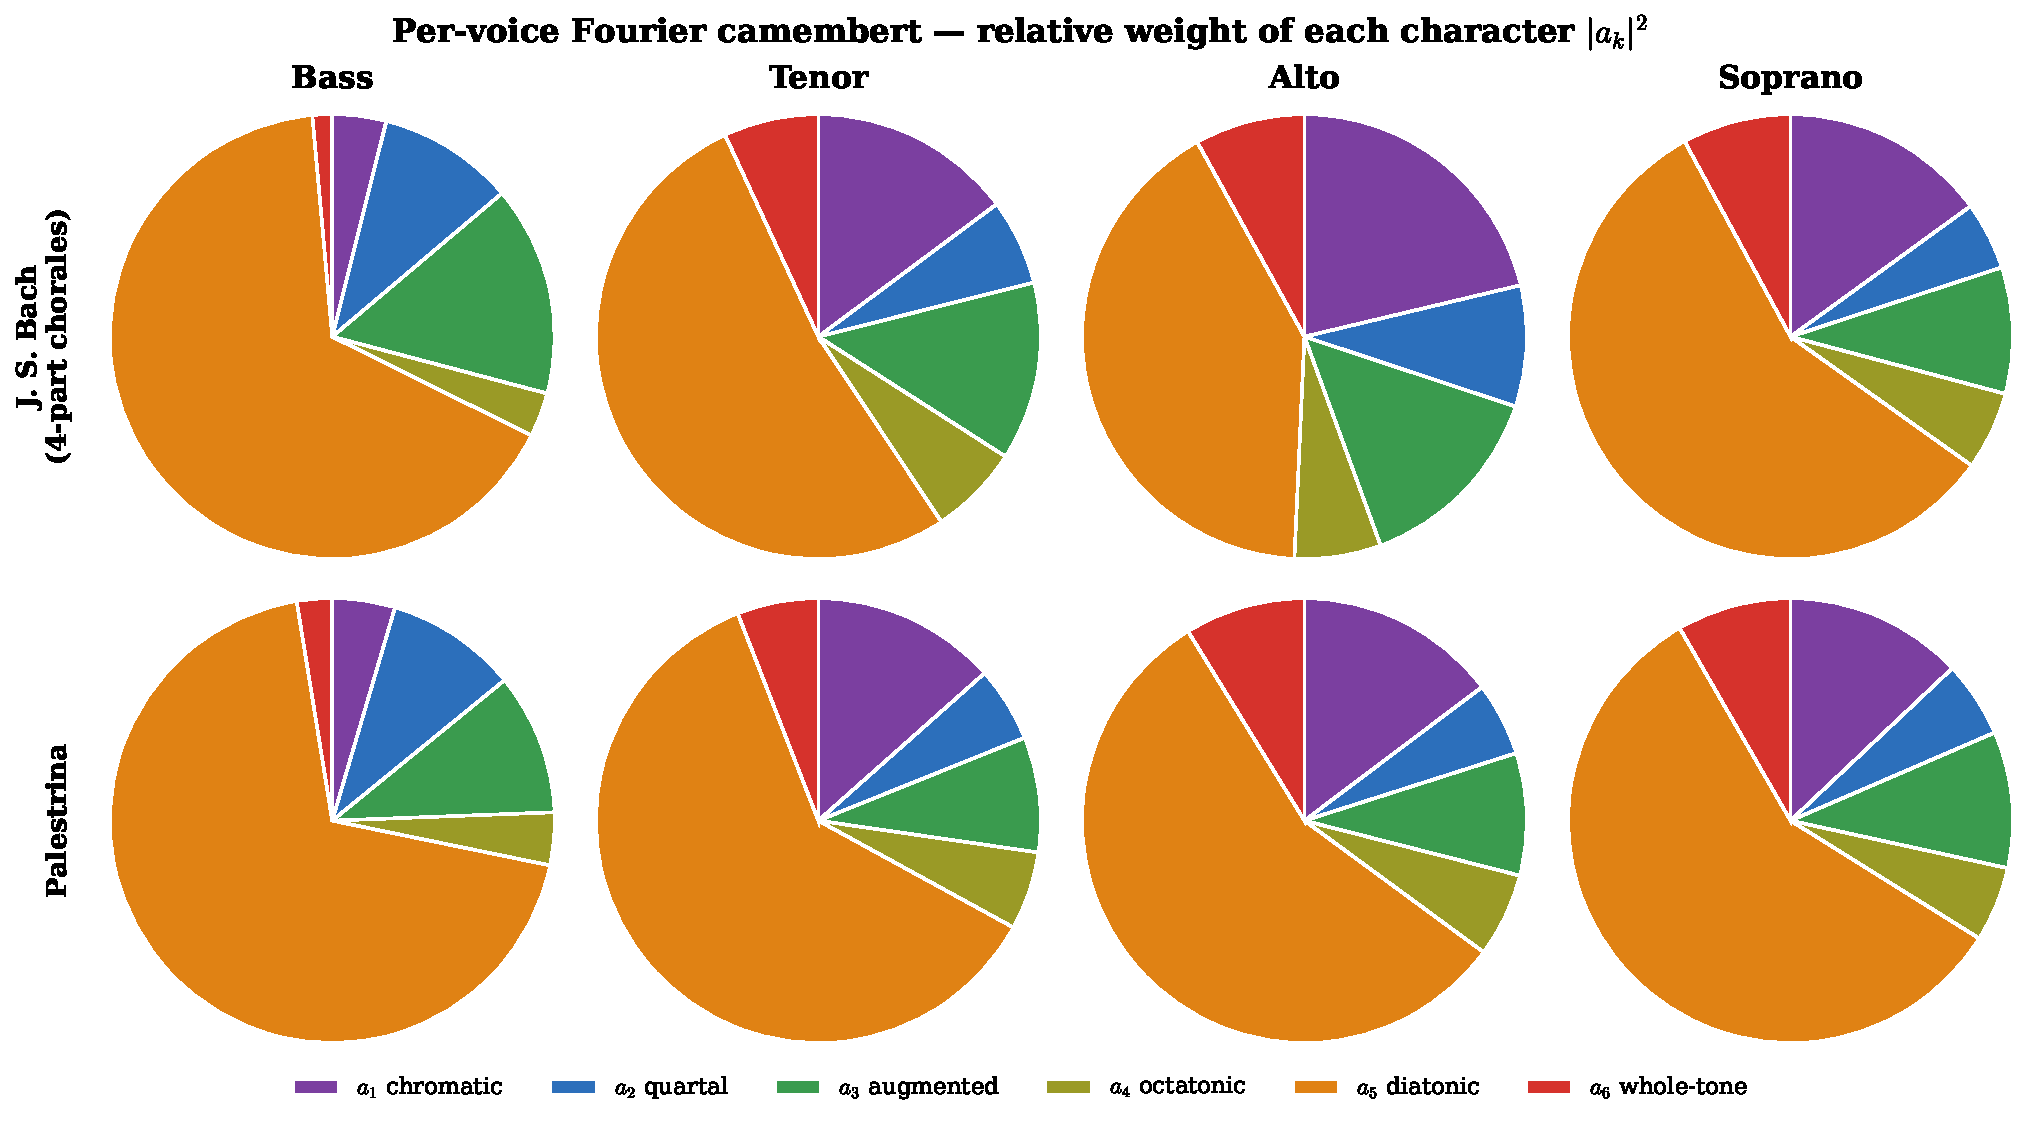
\includegraphics[width=\linewidth]{figs/fig1_camembert.pdf}
\caption{El ``camembert'' de Fourier por voz: el peso relativo de cada carácter ($|a_k|^2$, Parseval) para
Bajo/Tenor/Alto/Soprano, en corales de Bach (arriba) y Palestrina (abajo). El \textbf{sector del bajo} es
visiblemente fino en las porciones cromática (morado) y tono-entero (rojo) y grueso en diatónico (naranja);
el \textbf{alto} carga la mayor cuña cromática. La firma se lee de un vistazo y se reproduce en dos corpus
separados por dos siglos.}
\label{fig:camembert}
\end{figure}

\paragraph{No es un artefacto de cardinalidad.} Una distribución dispersa tiene coeficientes de alto $k$
pequeños, así que cabría sospechar que el bajo simplemente usa menos clases de altura. Es al revés: el bajo
usa \emph{más} clases de altura distintas que la soprano ($9{,}5$ frente a $7{,}5$ de media) y mayor
entropía, y aun así tiene el $\alpha_1$ más bajo. La baja cromaticidad es estructura distribucional
genuina, no un efecto de conteo.

\begin{figure}[H]\centering
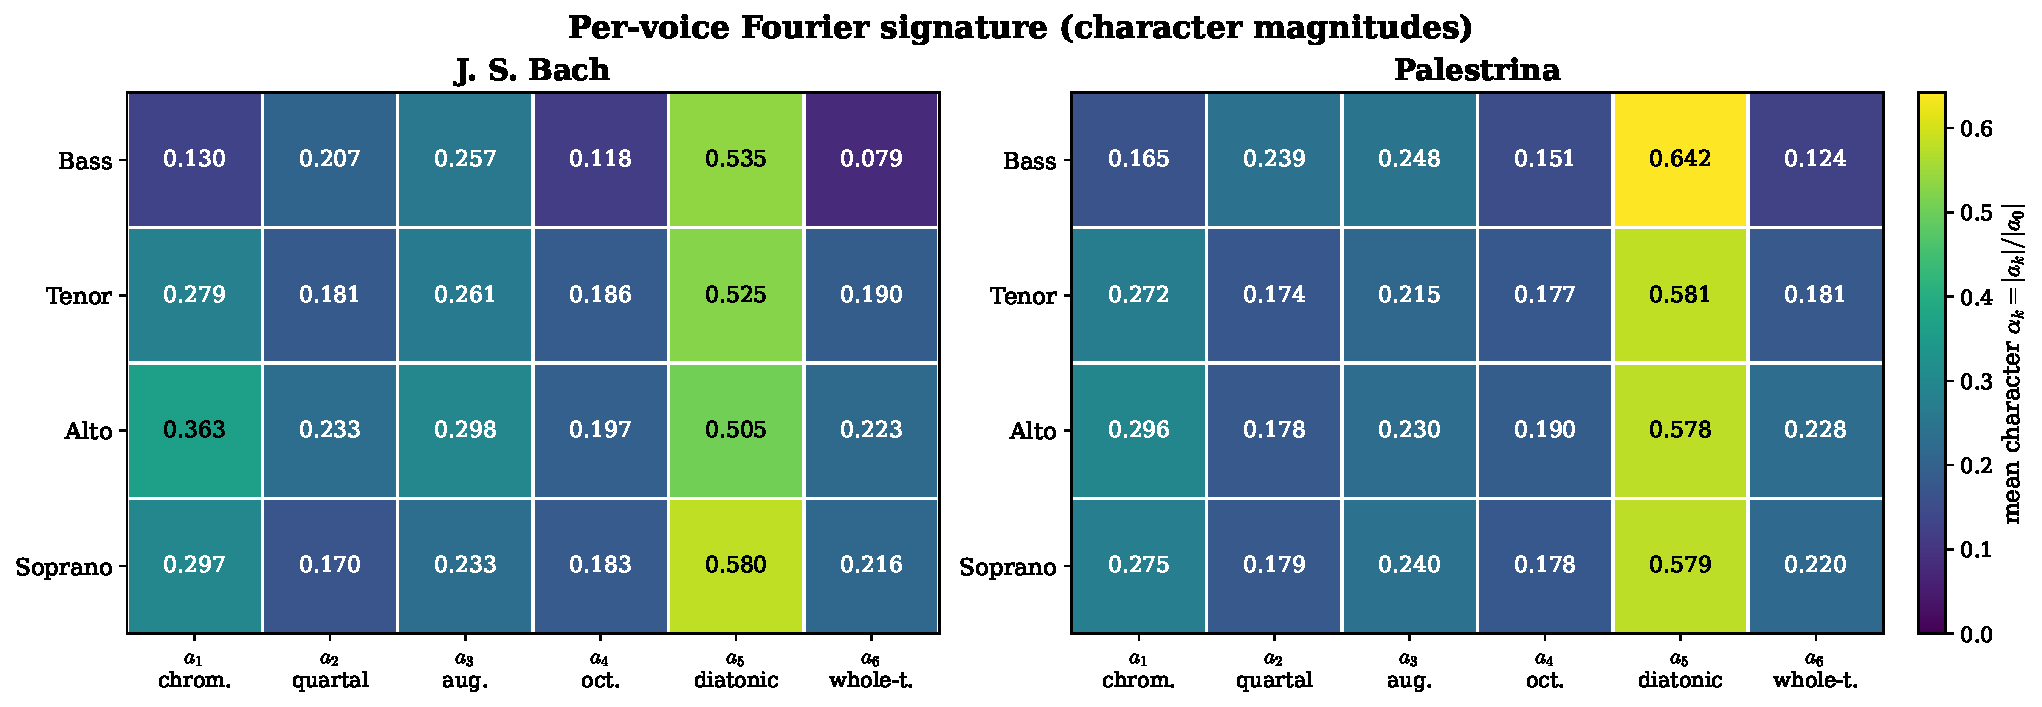
\includegraphics[width=\linewidth]{figs/fig7_heatmap.pdf}
\caption{La firma completa como matriz: voces $\times$ caracteres $\alpha_k$, Bach y Palestrina. La
\textbf{fila del bajo} es la más oscura en $a_1$ y $a_6$ y la más brillante en $a_5$, en ambos corpus; el
\textbf{alto} es el más brillante en $a_1$. La columna diatónica domina toda voz (música tonal/modal), pero
el \emph{contraste entre voces} vive en $a_1$ y $a_6$.}
\label{fig:heatmap}
\end{figure}

\section{El porqué: realización de raíces, en dos canales}\label{sec:why}

\question{P\textsubscript{2}. ¿Por qué es el bajo espectralmente puro ---y por qué en $a_1$ y $a_6$ en
particular?}

Porque, con una fidelidad de coseno del $95\%$ (ponderado por duración, Bach), la distribución del bajo
\emph{es} la distribución de las raíces de los acordes: el bajo realiza las raíces armónicas. El movimiento
funcional de raíces procede por quintas y cuartas ---intervalos $7$ y $5$, ambos \textbf{impares}. Este
único hecho impulsa dos canales espectrales distintos.

\paragraph{El canal de paridad ($a_6$).} El coeficiente de tono entero es, exactamente,
$a_6=\sum_{x}\mu(x)\,(-1)^x=(\text{peso par})-(\text{peso impar})$: lee la \textbf{imbalancia de paridad}
par/impar de la distribución (esta identidad es el núcleo certificado de la Sección~\ref{sec:checked}). Un
intervalo impar invierte la paridad de clase de altura; una progresión de raíces que camina por quintas
alterna entonces la paridad y \emph{equilibra} las dos colecciones de tono entero, enviando
$a_6\to0$\,\audio{arch_wholetone_highA6.wav}. Empíricamente, la correlación de $\alpha_6$ con la fracción de intervalos impares de la voz es de $-0{,}49$:
cuanto más se mueve una voz por intervalos impares (el bajo el que más), menor su tonalentereza.

\paragraph{El canal de dispersión ($a_1$).} El coeficiente $a_1$ mide el \emph{agrupamiento} cromático
---es grande cuando el peso se amontona en un arco contiguo del círculo cromático. El bajo funcional salta;
abarca la tesitura más amplia de las cuatro voces ($\approx 18$ semitonos frente a $\approx 12$), de modo
que su peso de clases de altura se dispersa ampliamente por el círculo en vez de agruparse, y $\alpha_1$ es
bajo\,\audio{arch_fifthchain_lowA1A6.wav}. Empíricamente, la correlación de $\alpha_1$ con el rango de la voz es de $-0{,}67$. La
Figura~\ref{fig:pcclock} lo muestra directamente: el peso del bajo se abre en abanico por el reloj, el del
alto se apiña en un arco.

\begin{figure}[H]\centering
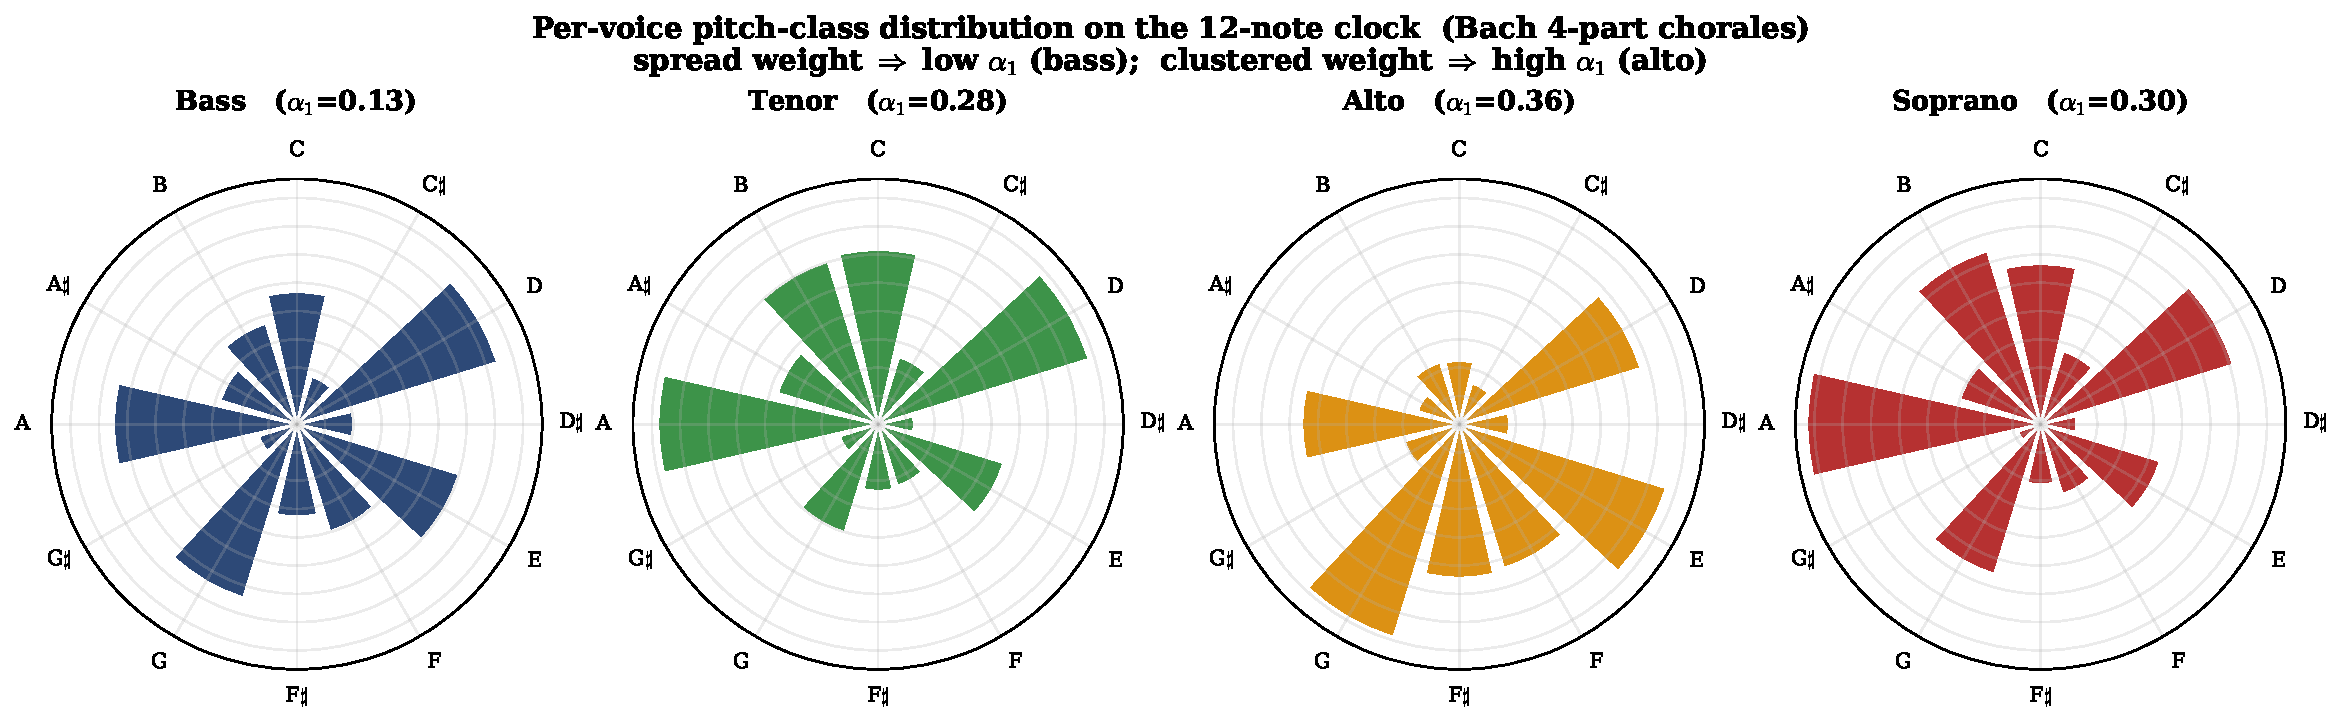
\includegraphics[width=\linewidth]{figs/fig5_pc_clock.pdf}
\caption{La distribución de clases de altura por voz dibujada sobre el reloj de doce notas (Bach). El
\textbf{bajo} ($\alpha_1=0{,}13$) dispersa su peso ampliamente por el círculo (bajo agrupamiento cromático);
el \textbf{alto} ($\alpha_1=0{,}36$) se apiña en un arco estrecho (alto agrupamiento). Peso disperso
$\Rightarrow$ $a_1$ bajo; peso agrupado $\Rightarrow$ $a_1$ alto ---el canal de dispersión, visto.}
\label{fig:pcclock}
\end{figure}

\paragraph{Un mecanismo que \emph{no} era la causa.} Es tentador atribuir la baja cromaticidad del bajo a
su movimiento melódico ---``el bajo evita los pasos de semitono''. No lo hace: la correlación de
$\alpha_1$ con la fracción de pasos melódicos de semitono es de solo $+0{,}01$, y el bajo tiene tantos
pasos de semitono como las otras voces. La causa está en la \emph{distribución} de clases de altura (qué
clases, cuán dispersas), no en la superficie melódica. Registramos el mecanismo refutado porque afila el
verdadero.

\section{El barrido histórico: un diagnóstico de la textura de bajo funcional}\label{sec:history}

\question{P\textsubscript{3}. Si la causa es el bajo funcional, la ley debería aparecer exactamente donde el
bajo porta raíces ---y desvanecerse donde no. ¿Lo hace?}

Lo hace ---y la forma más limpia de verlo es recorrer cuatro corpus a lo largo de cuatro siglos, cada uno
una relación distinta entre la voz más grave y la armonía. En el \textbf{Trecento} italiano (el \emph{Ars
Nova} del siglo XIV de Landini y sus contemporáneos) la polifonía se construye línea a línea sobre un
\emph{tenor} estructural; la voz más grave aún no es portadora de raíces armónicas, y la firma está
sencillamente ausente (el bajo es más puro que la voz aguda en $\alpha_1$ en el $52\%$ de las obras, en
$\alpha_6$ en el $58\%$ ---ni mejor que la moneda al aire del $50\%$). Para el \textbf{stile antico} de
Palestrina (contrapunto modal del siglo XVI, la música de la Contrarreforma) una voz más grave clara ya
gobierna la implicación armónica de cada sonoridad, y la firma es fuerte ($87\%$, $77\%$). Vuelve a ser
fuerte dos siglos después en los corales de \textbf{Bach} ($85\%$, $73\%$) ---la apoteosis de la armonía
funcional a cuatro voces, donde el bajo sencillamente \emph{es} el fundamento del bajo cifrado de
\S\ref{sec:hook}. El caso revelador es \textbf{Monteverdi}: sus madrigales son \emph{posteriores} a
Palestrina y sin embargo muestran el efecto \emph{más débil} ($65\%$, $53\%$ ---cerca del azar), porque el
expresivo madrigal de la \emph{seconda prattica} es imitativo y guiado por el texto, repartiendo su color
cromático entre cinco voces casi iguales en las que ninguna línea es la portadora privilegiada de raíces.
Así, la firma rastrea la \textbf{textura, no la fecha} (Figura~\ref{fig:sweep}): es fuerte exactamente
donde el bajo realiza raíces y se desvanece donde no. El límite no es un fallo de la ley sino su
confirmación ---el mismo mecanismo de realización de raíces que predice el efecto predice dónde debe
desaparecer--- y reencuadra el efecto como un \textbf{diagnóstico de la escritura de bajo funcional}, una
huella espectral de la práctica misma que Rameau teorizó.

\begin{figure}[H]\centering
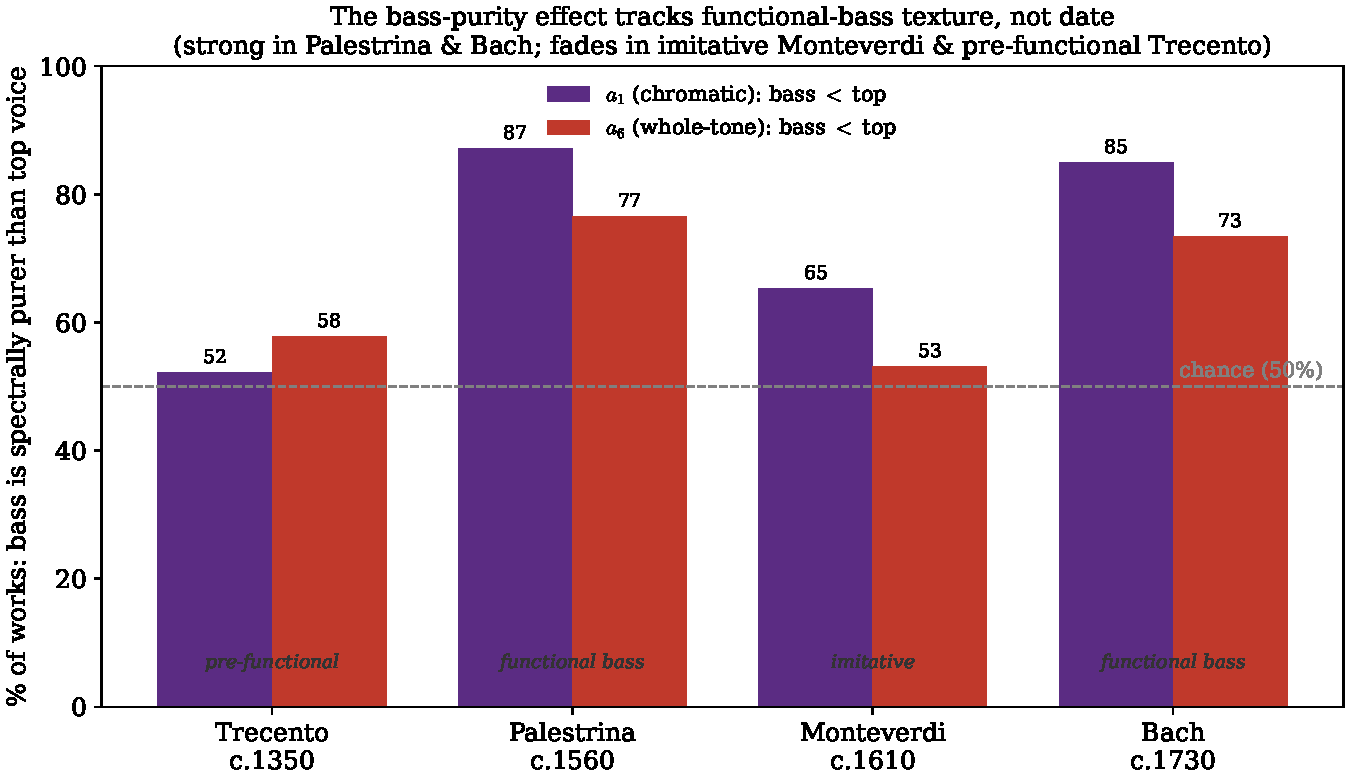
\includegraphics[width=0.92\linewidth]{figs/fig9_historical_sweep.pdf}
\caption{El efecto de pureza del bajo a través de cuatro corpus. Barras: porcentaje de obras en que el bajo
es espectralmente más puro que la voz aguda, en $a_1$ (cromático) y $a_6$ (tono entero), frente a la línea
de azar del $50\%$. Fuerte en la homofonía de bajo funcional (Palestrina, Bach), se desvanece en texturas
imitativas (Monteverdi) y prefuncionales (Trecento) ---rastreando el papel del bajo, no la cronología.}
\label{fig:sweep}
\end{figure}

\section{El dual: las voces internas llevan el color}\label{sec:dual}

\question{P\textsubscript{4}. Si el bajo es el más puro, ¿cuál es la voz menos pura ---y por qué?}

El orden de cromaticidad es Bajo $0{,}130<$ Tenor $0{,}279<$ Soprano $0{,}297<$ \textbf{Alto $0{,}363$}:
las voces internas, el alto sobre todo, llevan el color más cromático\,\audio{arch_chromatic_highA1.wav}. Es el canal de dispersión al revés:
las voces internas ocupan la tesitura \emph{más estrecha} ($\approx 11$--$12$ semitonos), de modo que su
peso se comprime en una banda cromática y $\alpha_1$ es alto. Es la historia de la dispersión registral, no
una de cromaticidad melódica (la correlación con los pasos de semitono es nula, como en \S\ref{sec:why}).
Las cuatro voces se sitúan, en el plano de fase diatónica $(\Phi_3,\Phi_5)$, casi unas sobre otras
(Figura~\ref{fig:phaseplane}) ---comparten tonalidad--- de modo que la información entre voces está en las
\emph{magnitudes} $\alpha_1,\alpha_6$, no en las fases: un bajo y una soprano difieren en \emph{pureza}
espectral, no en centro tonal.

Esto invierte la imagen de manual de un modo preciso. Las voces \emph{externas} son el marco estructural
---el bajo enraizando la armonía, la soprano llevando la melodía--- mientras que las voces \emph{internas}
son donde vive el color cromático: el hogar de las retardos, las notas de paso y bordadura, y la pequeña
conducción cromática que rellena una textura a cuatro voces. Que el alto sea la voz más cromática de todas
es así el eco espectral de una práctica tan antigua como el \emph{altus} de la polifonía renacentista ---las
partes internas se mueven por los pasos cortos, a menudo cromáticos, que el bajo, saltando por quintas,
nunca da, y que la soprano, cantando la melodía diatónica, evita en su mayoría. Pureza abajo, melodía
arriba, color dentro: los caracteres de Fourier recuperan la división del trabajo del propio coral a cuatro
voces.

\begin{figure}[H]\centering
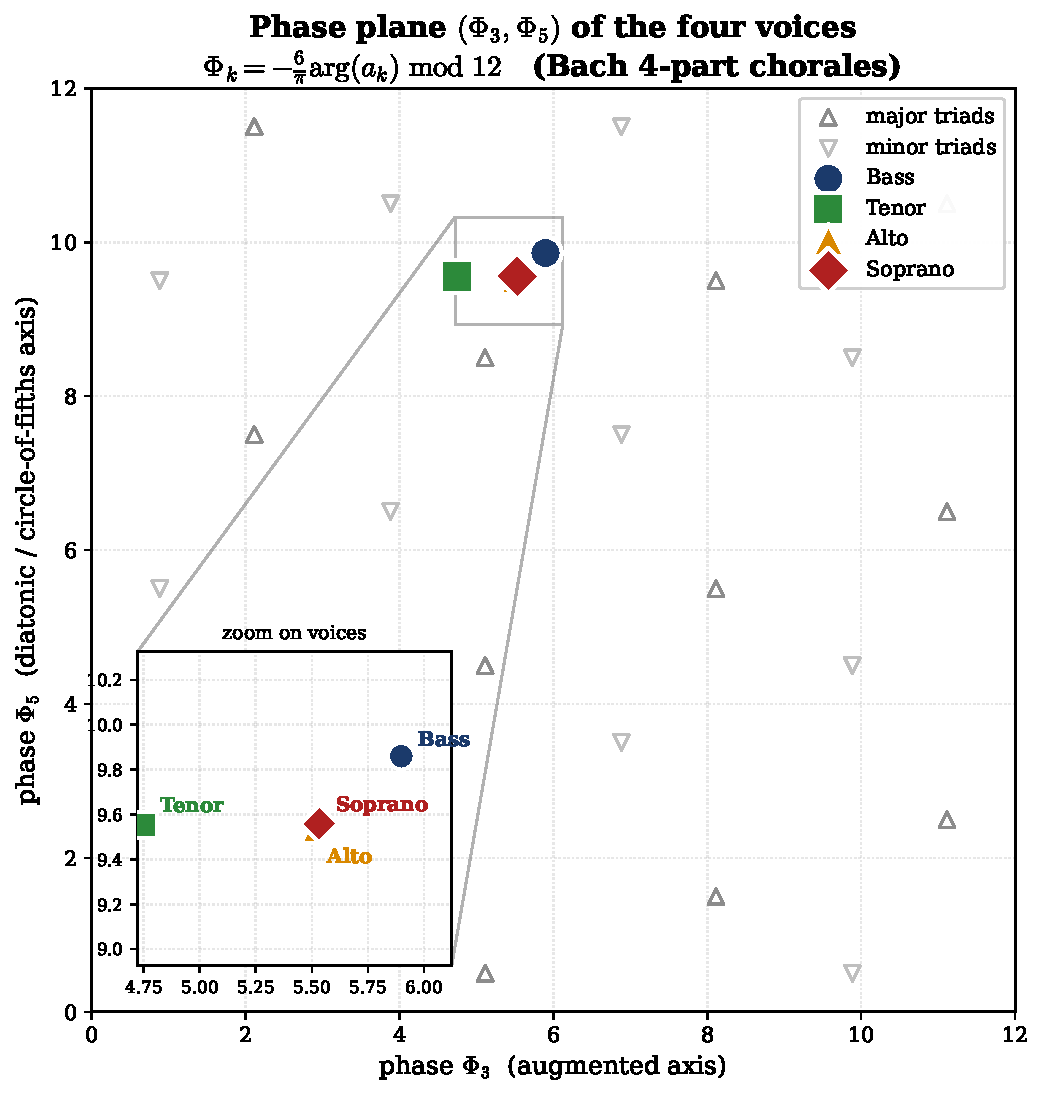
\includegraphics[width=0.50\linewidth]{figs/fig6_phase_plane.pdf}
\caption{Las cuatro voces en el plano de fase diatónica $(\Phi_3,\Phi_5)$ frente a las $24$ tríadas
mayores/menores. Las voces son casi coincidentes (una tonalidad compartida): el contraste por voz lo llevan
las \emph{magnitudes} de carácter ($a_1,a_6$), no las fases.}
\label{fig:phaseplane}
\end{figure}

\section{Lo que está verificado por máquina}\label{sec:checked}

\question{P\textsubscript{5}. La ley empírica descansa en una medición; ¿qué parte está certificada?}

El núcleo del canal de paridad ---la identidad que hace del coeficiente de tono entero un recuento de
paridad--- está probado en Lean~4 (\lean{ParityA6.lean}, espacio de nombres \lean{ParityA6}, sin
\lean{sorry}; construido sobre el \lean{Fourier.lean} del proyecto). La Tabla~\ref{tab:lean} lista los
resultados. Lo central es que $a_6$ \emph{es} la imbalancia de paridad par-menos-impar, con la frecuencia
de orden $2$ leyendo paridad en \emph{cualquier} universo par $\Zn{2m}$, no solo $\Ztwelve$. La auditoría de
axiomas (\lean{\#print axioms}) devuelve a lo sumo \lean{[propext, Classical.choice, Quot.sound]} en todo
resultado nombrado ---sin \lean{sorryAx}, sin \lean{Lean.ofReduceBool}--- confirmado recompilando en el
entorno de bucle rápido del proyecto (EXIT~0).

\begin{table}[H]
\centering\small
\rowcolors{2}{ctA!7}{white}
\begin{tabular}{@{}l p{0.56\textwidth}@{}}
\toprule
\rowcolor{ctA!22}
\textbf{Resultado Lean (\lean{ParityA6.lean})} & \textbf{Enunciado}\\
\midrule
\lean{Ahat\_six\_eq\_sum\_neg\_one\_pow} & $\Ahat(6)=\sum_{x\in A}(-1)^{x}$ --- el coeficiente de tono entero es la suma de paridad con signo.\\
\lean{Ahat\_six\_eq\_card\_sub} & $\Ahat(6)=\#(\text{cl.\ pares})-\#(\text{cl.\ impares})$ --- la imbalancia de paridad, sobre $\mathbb{C}$.\\
\lean{Ahat\_six\_eq\_zero\_iff} & $\Ahat(6)=0\iff \#(\text{pares})=\#(\text{impares})$ --- $a_6$ se anula exactamente en el equilibrio par/impar.\\
\lean{dftN\_half\_eq\_sum\_neg\_one\_pow} & Universo par general: en $\Zn{2m}$, la frecuencia de orden $2$ lee paridad, $\hat\mu(m)=\sum_x(-1)^{x}$.\\
\bottomrule
\end{tabular}
\caption{El núcleo de paridad del canal $a_6$, verificado por máquina. Lo acompañan cuatro testigos
\lean{example} (Do mayor $a_6=1$; tono entero $a_6=6$; diatónica $a_6=-1$; un tetracordo equilibrado
$a_6=0$). La matemática es clásica (véase \S\ref{sec:novelty}); esta es su primera formalización.}
\label{tab:lean}
\end{table}

\section{Novedad, alcance, y lo que esta nota no afirma}\label{sec:novelty}

\paragraph{Contribución, dicha con claridad.} Esta es una nota \textbf{empírica} con un \textbf{núcleo
formalizado}, no matemática nueva. Todo ingrediente explicativo es clásico: el bajo funcional es
Rameau~\cite{Rameau} y Riemann~\cite{Riemann}; el programa de la DFT-de-distribuciones y las lecturas de
caracteres ($a_5=$ diatonicidad, etc.) son Lewin~\cite{Lewin1959}, Quinn~\cite{Quinn}, Amiot~\cite{Amiot},
Yust~\cite{Yust2017,Yust2019}; la identidad $a_6=$ paridad de clases es Amiot (\emph{The Torii of
Phases}~\cite{Torii}, ``$a_6$ toma solo dos valores, según el número de alturas impares''), y el mecanismo
del movimiento de una sola nota detrás de ella es Hoffman~\cite{Hoffman}. \textbf{El contenido nuevo es la
ley de magnitud por voz}: que, en texturas de bajo funcional, el bajo es la voz espectralmente más pura (el
$\alpha_1,\alpha_6$ más bajos), medido en corpus, explicado por la realización de raíces en dos canales, y
acotado por la textura. El programa de la DFT lee texturas por \emph{tiempo}; el contraste de magnitud por
voz (registral) es el corte ortogonal, y está, según nuestra búsqueda, sin enunciar.

\paragraph{Lo que esta nota \emph{no} afirma.}
\begin{itemize}\itemsep2pt
  \item \textbf{No es un teorema.} La ley es una regularidad empírica; su núcleo matemático es la
        linealidad de la DFT sobre la descomposición en voces. Solo la identidad de paridad
        (Tabla~\ref{tab:lean}) es un teorema en Lean.
  \item \textbf{No es universal.} La firma es un diagnóstico de la textura de \emph{bajo funcional}: fuerte
        en Palestrina y Bach, débil/ausente en madrigales de Monteverdi y en el Trecento
        (\S\ref{sec:history}).
  \item \textbf{No es la conjetura de la diatonicidad.} El bajo \emph{no} es la voz más diatónica ($a_5$);
        esa es la soprano. El invariante es el $a_1$ y $a_6$ bajos del bajo, no un $a_5$ alto.
  \item \textbf{No es una afirmación melódica.} La baja cromaticidad es una propiedad de la
        \emph{distribución} de clases de altura (dispersión / paridad), no del movimiento melódico de
        semitono (correlación $+0{,}01$).
  \item \textbf{No es prioridad sobre el programa de la DFT.} Lewin, Quinn, Amiot y Yust preceden a esto;
        citamos, medimos, formalizamos y no suplantamos. La identidad de paridad es de Amiot/Hoffman;
        nuestro \lean{ParityA6.lean} es su primera formalización, y es \emph{distinta} de ---no un corolario
        de--- el lema del tritono de Amiot (que concierne a los coeficientes de índice \emph{impar}).
\end{itemize}

\paragraph{Frontera abierta.} Un corpus mayor y más estilos cartografiarían el límite de textura con
precisión (¿dónde, cuantitativamente, empieza el ``bajo funcional''?); un estudio por voz de las
\emph{fases} (en vez de las magnitudes) queda intacto aquí; y el canal de dispersión invita a un enunciado
limpio que acote $a_1$ por la dispersión circular de una voz.

\section*{Disponibilidad de datos y código}
Las mediciones por voz (\lean{music21}: $334$ corales de Bach a cuatro voces, $367$ obras de Palestrina,
más los corpus de Monteverdi y Trecento), el conjunto de figuras (\lean{voice\_figs.py}, que regenera las
Figuras~\ref{fig:camembert}--\ref{fig:phaseplane} desde los corpus), las sonificaciones
(\lean{media/}) y la fuente Lean \lean{ParityA6.lean} acompañan esta nota; cada resultado Lean es
comprobable con \lean{\#print axioms} y cada script es reejecutable.

\begin{thebibliography}{99}
\bibitem{Rameau} J.-Ph. Rameau, \emph{Trait\'e de l'harmonie r\'eduite \`a ses principes naturels},
  Ballard, Paris, 1722.
\bibitem{Riemann} H. Riemann, \emph{Vereinfachte Harmonielehre}, Augener, London, 1893.
\bibitem{Lewin1959} D. Lewin, ``Re: Intervallic relations between two collections of notes,''
  \emph{J. Music Theory} \textbf{3} (1959), no.~2, 298--301.
\bibitem{Quinn} I. Quinn, ``General equal-tempered harmony,'' \emph{Perspectives of New Music}
  \textbf{44}/2--\textbf{45}/1 (2006--2007).
\bibitem{Amiot} E. Amiot, \emph{Music Through Fourier Space: Discrete Fourier Transform in Music Theory},
  Computational Music Science, Springer, 2016.
\bibitem{Torii} E. Amiot, ``The Torii of phases,'' in \emph{Mathematics and Computation in Music}
  (MCM 2013), LNCS \textbf{7937}, Springer (2013), pp.~1--18; arXiv:1208.4774.
\bibitem{Yust2017} J. Yust, ``Probing questions about keys: tonal distributions through the DFT,'' in
  \emph{Mathematics and Computation in Music} (MCM 2017), LNCS \textbf{10527}, Springer (2017),
  pp.~167--179.
\bibitem{Yust2019} J. Yust, ``Stylistic information in pitch-class distributions,'' \emph{J. New Music
  Research} \textbf{48} (2019), no.~3, 217--231.
\bibitem{TY} D. Tymoczko, J. Yust, ``Fourier phase and pitch-class sum,'' in \emph{Mathematics and
  Computation in Music} (MCM 2019), LNCS \textbf{11502}, Springer (2019), pp.~46--58.
\bibitem{Hoffman} J. Hoffman, ``On pitch-class set cartography: relations between voice-leading and
  Fourier spaces,'' \emph{J. Music Theory} \textbf{52} (2008), no.~2, 219--249.
\bibitem{Cohn} R. Cohn, ``Maximally smooth cycles, hexatonic systems, and the analysis of late-Romantic
  triadic progressions,'' \emph{Music Analysis} \textbf{15} (1996), no.~1, 9--40.
\bibitem{m21} M. Cuthbert, C. Ariza, ``music21: a toolkit for computer-aided musicology and symbolic music
  data,'' \emph{ISMIR} (2010), 637--642.
\end{thebibliography}

\end{document}
